\chapter{JPEG 图像有损压缩}
JPEG(Joint Photographic Experts Group,联合图像专家组),是一种常用的图像存储格式,是一种高效率的压缩格式,文件格式是JPEG(联合图像专家组)标准的产物,该标准由ISO与CCI TT(国际电报电话咨询委员会)共同制定,是面向连续色调静止图像的一种压缩标准。

JPEG有损图像压缩主要包括图像分块、颜色空间转换、色度采样、离散余弦变换DCT、量化、编码等步骤。

\section{图像分块}
在JPEG流程中,对整张图像进行一步压缩不太现实,首先是算法的复杂度较大需要大量消耗计算资源,其次,如果图像较大,甚至无法进行处理,因此原始图像会被分割成大小为$8\times 8$的图像子块,在后续的压缩编码处理中,会以图像子块为单位进行处理。

\section{颜色空间转换与色度采样}
\subsection{颜色空间转换与色度采样的理论基础}

在人眼视觉系统(Human Visual System, HVS)理论\cite{HVS}中,对光线的感知主要依靠视网膜上的细胞,在视网膜上两种感光细胞,一种叫做视锥细胞,另—种叫做视杆细胞。一只眼睛里面大约分别有七百万视锥细胞和一亿两千万视杆细胞。

视锥细胞(cone cell)负责感知较强的光照和色彩,视网膜中有三种视锥细胞,它们有重叠的频率响应曲线,但响应强度有所不同,分别对红(570nm), 绿(535nm), 蓝(445nm)光有最敏感,共同决定了人眼对色彩的感觉。

视杆细胞(rod cell)只能感知光照而不能感知色彩,在视网膜中只有一种视杆细胞,因此没有颜色感觉,但对光的灵敏度非常高,可以看到非常暗的物体,这也就是人眼在暗光下无法分辨颜色的原因。

由于主要感知光照视杆细胞的数量远远多于主要感知色彩的视锥细胞,因此人眼对光照的变化会比对颜色的变化更加敏感,图像有损压缩的主要根据此特性来对颜色(色度)进行进一步采样来压缩图像以减少图像数据中的冗余部分,该冗余指的是无法被人眼所感知的部分。

根据人眼的这一特点,在图像和视频编码中,保留色度信息,大幅度对色度进行采样的技术有着十分广泛的应用,尤其是在视频编码中通过减少色度信息保留亮度信息以降低视频带宽。同样的,JPEG标准中也根据此特点对色度进行采样。

\subsection{颜色空间转换}
根据上述理论基础,在JPEG标准中,首先将 RGB 颜色空间转化为 YUV 颜色空间(也叫 YCbCr)其中,Y 是亮度 (Luminance)(也叫亮度信息),U 和 V 表示色度 (Chrominance)(也叫色差信息)。

研究表明,红绿蓝三基色所贡献的亮度不同,绿色所贡献亮度最多,蓝色所贡献亮度最少,这是由于人眼对相同强度不同波长的光具有不同的敏感度,其中对绿色光(550nm)产生最大的光强敏感度,而对蓝色光(445nm)产生光强敏感度较小。假定红色贡献为 $K_R$,蓝色贡献为 $K_B$,则亮度可以表示为

\begin{equation}
    Y = K_R \cdot R + (1-K_R-K_B) \cdot G + K_B \cdot B
    \label{Eq.yuv}
\end{equation}

根据经验值 $K_R=0.299, K_B=0.114$,则有
\begin{equation}
    Y = 0.299 \cdot R + 0.587 \cdot G + 0.114 \cdot B
\end{equation}

蓝色和红色的色差为
\begin{equation}
    \begin{aligned}
        Y   &= 0.299   \cdot R + 0.587    \cdot G + 0.114 \cdot B \\
        C_b &= -0.1687 \cdot R - 0.3313   \cdot G + 0.5 \cdot B +128\\
        C_r &= 0.5   \cdot R - 0.4187   \cdot G - 0.0813 \cdot B +128\\
    \end{aligned}    
\end{equation}

矩阵表示为
\begin{equation}
    \begin{bmatrix}
        Y \\ C_b \\ C_r
    \end{bmatrix}
    =\begin{bmatrix}
        0.299   & 0.587    & 0.114 & \\
        -0.1687 & -0.3313   & 0.5 & \\
        0.5     & -0.4187   & -0.0813 &
    \end{bmatrix}
    \begin{bmatrix}
        R \\ G \\ B
    \end{bmatrix}
    +\begin{bmatrix}
        0 \\ 128 \\ 128
    \end{bmatrix}
\end{equation}


\subsection{色度采样}
将 RGB 颜色空间转化为 YUV 颜色空间后,需要对色度进行二次采样,从而进一步压缩图像数据中不容易被人眼感知的冗余部分。YUV色彩空间下的色度采样主要有三种采样方式,分别是4:4:4采样、4:4:2采样、4:2:0采样。

三种色度采样方式在图\ref{Fig.chrominance_sample}中示例,其中,$J$表示水平抽样参照(概念上区域的宽度,通常为4),$a$表示在J个像素第一行中的色度抽样数目(Cr, Cb),$b$表示在J个像素第二行中的额外色度抽样数目(Cr, Cb)。

4:4:4采样。第一行中,每连续4个点采样4个 CrCb 值,第二行中,每连续4个点采样4个 CrCb 值,即每一个Y对应一个Cr和一个Cb。图像数据中的色度信息完整保留。

4:4:2采样。第一行中,每连续4个点采样2个 CrCb 值,第二行中,每连续4个点采样4个 CrCb 值,即每两个Y共用一对Cr和Cb。图像数据中的仅有50\%的色度信息保留。许多高端数字视频格式和接口都使用这种方案,包括流行的 Apple ProRes422 编码\cite{AppleproResWhiteBook}。

4:2:0采样。第一行中,每连续4个点采样2个 CrCb 值,第二行中,不采样 CrCb ,沿用第一行的 CrCb 值,即每四个Y共用一对Cr和Cb。图像数据中的仅有25\%的色度信息保留。


\begin{figure}[!htb]
    \centering
    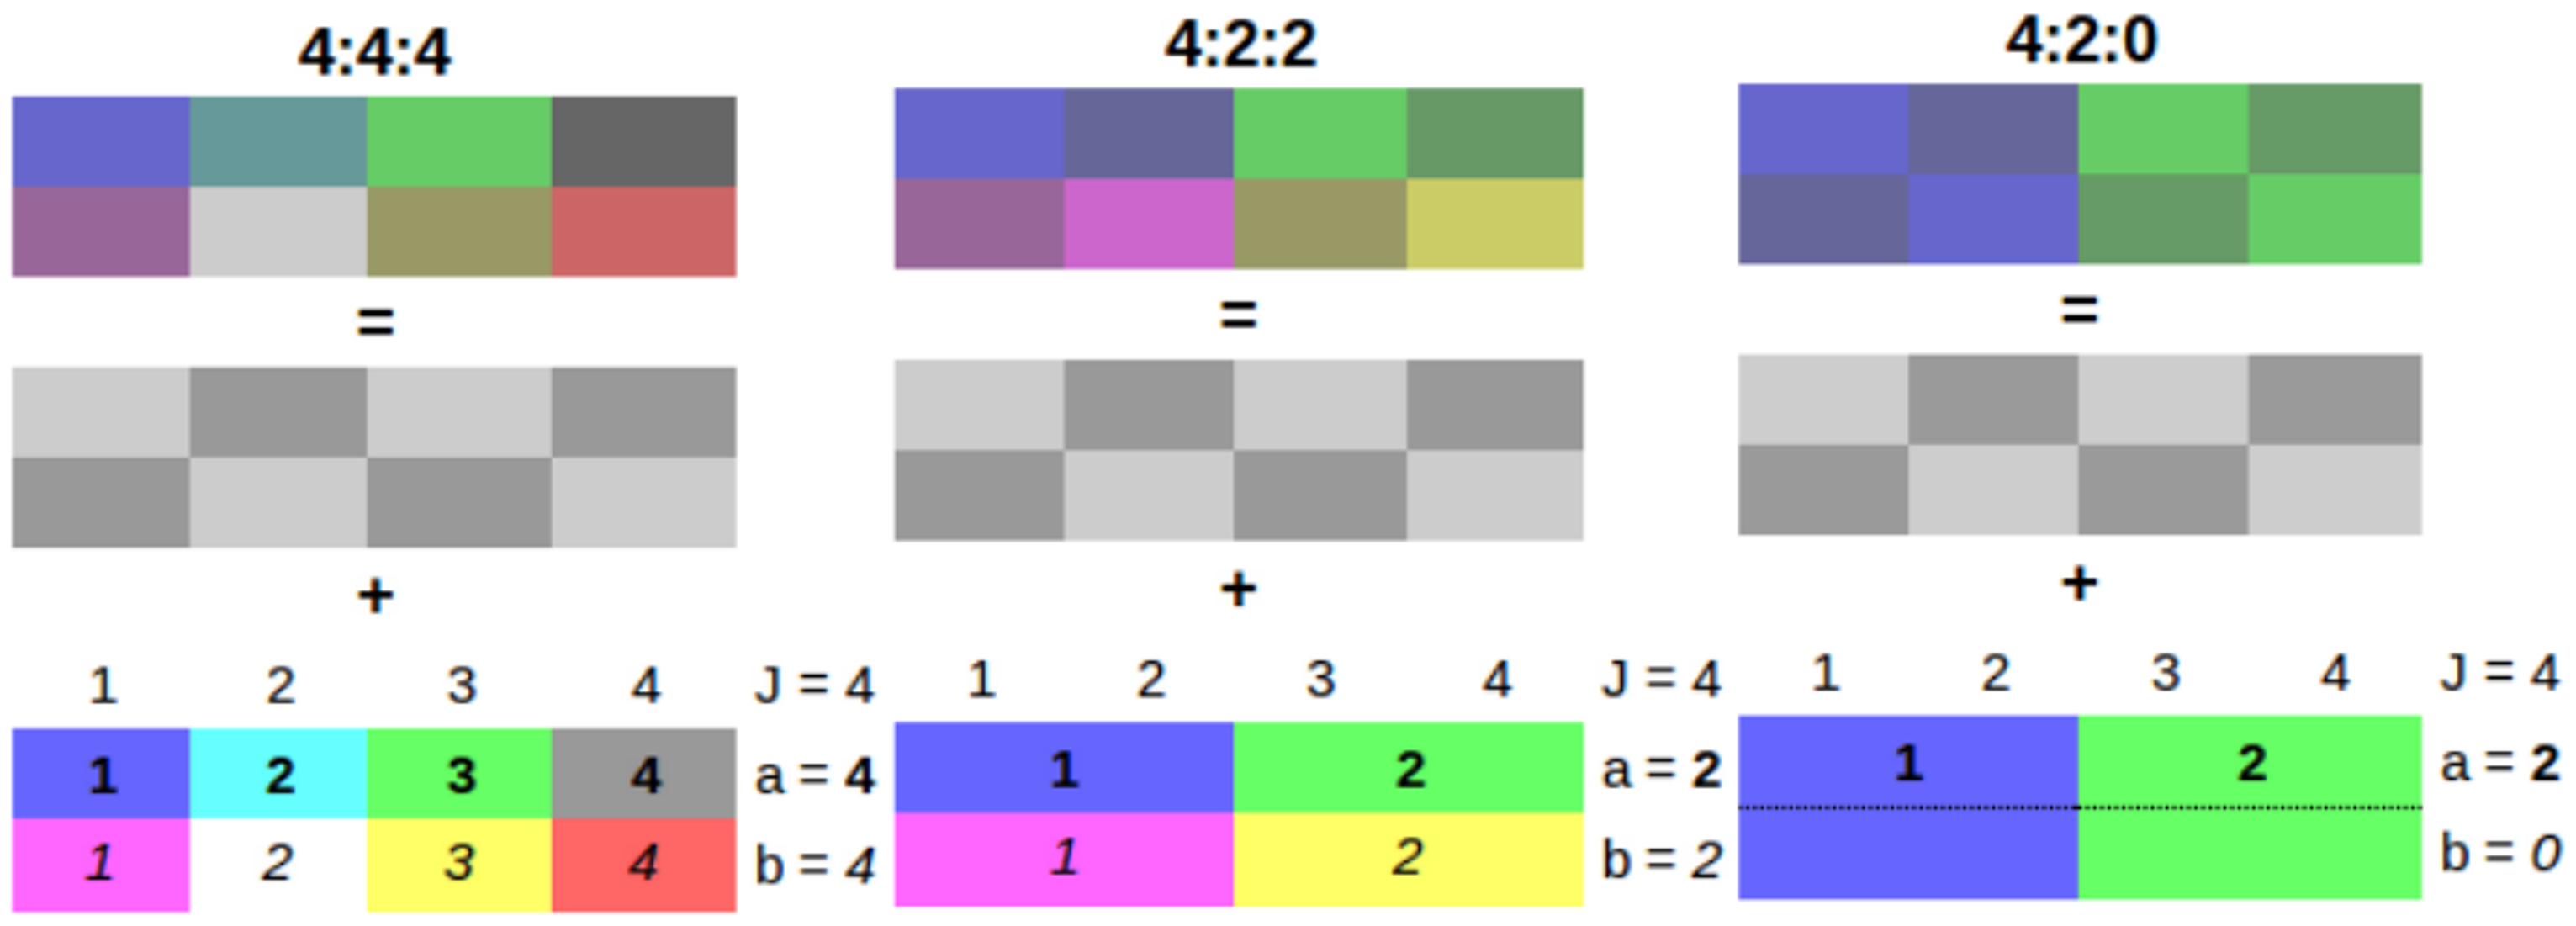
\includegraphics[width=1.0\textwidth]{pages/jpeg/chrominance_sample.png}
    \caption{3种色度采样示例}
    \label{Fig.chrominance_sample}
\end{figure}


\section{DCT变换}
离散余弦变换(Discrete Cosine Transform,DCT)能够将空域的信号转换到频域上,具有良好的去相关性的性能。DCT变换本身是无损的且具有对称性。对原始图像进行离散余弦变换,变换后DCT系数能量主要集中在左上角,其余大部分系数接近于零。将变换后的DCT系数进行门限操作,将小于一定值得系数归零,这就是图像压缩中的量化过程,然后进行逆DCT运算,可以得到压缩后的图像。

对原始图像信号$f(i,j)$进行二维DCT变换得到频域信号$F(u,v)$

\begin{equation}
    \begin{aligned}
        F(u,v) &=c(u)c(v) \sum_{i=0}^{M-1} \sum_{j=0}^{N-1} f(i,j) \cos(\frac{i+0.5}{M}u\pi) \cos(\frac{j+0.5}{N}u\pi) \\
        c(u) &=\left\{\begin{aligned}
            & \sqrt{\frac{1}{N}}, & \quad u=0 \\
            & \sqrt{\frac{2}{N}}, & \quad u\neq 0
        \end{aligned}\right.
        \quad u,v=0,1,2,...,7
    \end{aligned}
\end{equation}
当 $M=N$ 时,即对方阵进行 DCT 变换时,DCT 变换可以用DCT矩阵进行简化计算, $f$ 的 DCT 变换则是 $F=TfT^T$,其中 DCT 变换矩阵 $T$ 为
\begin{equation}
    T=\frac{2}{\sqrt{N}}
    \begin{bmatrix}
        \frac{1}{\sqrt{2}}      & \frac{1}{\sqrt{2}}        & ...   & \frac{1}{\sqrt{2}} \\
        \cos\frac{\pi}{2N}      & \cos\frac{3\pi}{2N}       & ...   & \cos\frac{(2N-1)\pi}{2N} \\
        ...                     & ...                       &       & ... \\
        \cos\frac{(N-1)\pi}{2N} & \cos\frac{3(N-1)\pi}{2N}  & ...   & \cos\frac{(2N-1)(N-1)\pi}{2N}
    \end{bmatrix}
\end{equation}


当原始图像从 RGB 颜色空间转换到 YUV 颜色空间之后,需要对每一个 $8 \times 8$ 的图像块进行二维DCT变换
\begin{equation}
    \begin{aligned}
        F(u,v) &=c(u)c(v) \sum_{i=0}^{7} \sum_{j=0}^{7} f(i,j) \cos(\frac{i+0.5}{8}u\pi) \cos(\frac{j+0.5}{8}u\pi) \\
        c(u) &=\left\{\begin{aligned}
            & \sqrt{\frac{1}{8}},   & \quad u=0 \\
            & \frac{1}{2},          & \quad u\neq 0
        \end{aligned}\right.
        \quad u,v=0,1,2,...,7
    \end{aligned}
\end{equation}

由于图像子块是方阵,这时候的 DCT 变换矩阵 $T$ 为
\begin{equation}
    T=\frac{1}{\sqrt{2}}
    \begin{bmatrix}
        \frac{1}{\sqrt{2}}      & \frac{1}{\sqrt{2}}        & ...   & \frac{1}{\sqrt{2}} \\
        \cos\frac{\pi}{16}      & \cos\frac{3\pi}{16}       & ...   & \cos\frac{(16-1)\pi}{16} \\
        ...                     & ...                       &       & ... \\
        \cos\frac{(N-1)\pi}{16} & \cos\frac{3(N-1)\pi}{16}  & ...   & \cos\frac{(16-1)(N-1)\pi}{16}
    \end{bmatrix}
\end{equation}

在 Matlab 中可以用 \lstinline|T = dctmtx(8)| 查看

\begin{lstlisting}{Matlab}
T =
  0.3536  0.3536  0.3536  0.3536  0.3536  0.3536  0.3536  0.3536
  0.4904  0.4157  0.2778  0.0975 -0.0975 -0.2778 -0.4157 -0.4904
  0.4619  0.1913 -0.1913 -0.4619 -0.4619 -0.1913  0.1913  0.4619
  0.4157 -0.0975 -0.4904 -0.2778  0.2778  0.4904  0.0975 -0.4157
  0.3536 -0.3536 -0.3536  0.3536  0.3536 -0.3536 -0.3536  0.3536
  0.2778 -0.4904  0.0975  0.4157 -0.4157 -0.0975  0.4904 -0.2778
  0.1913 -0.4619  0.4619 -0.1913 -0.1913  0.4619 -0.4619  0.1913
  0.0975 -0.2778  0.4157 -0.4904  0.4904 -0.4157  0.2778 -0.0975
\end{lstlisting}

对图像进行 $8\times 8$ 分块后,对每一个图像子块(patch)矩阵块 P 都进行 DCT 变换 $TPT^T$ 就可以将图像子块从空域变换到频域,从而在频域对图像进行压缩。

\section{量化}
\section{熵编码}
\subsection{霍夫曼编码}
霍夫曼编码是一种用于无损数据压缩的熵编码(权编码)算法,其使用变长编码表对数据进行编码。

变长编码表是通过评估符号出现概率得到的,出现概率高的符合使用较短的编码,反之出现概率低的则使用较长的编码,使编码之后的字符串的平均长度降低,从而达到无损压缩数据的目的。

霍夫曼编码主要分为两步:

根据每个字符出现的概率构建一颗最优二叉树;

再根据二叉树对字符进行编码。
